\section{Our Method}
\begin{wrapfigure}{r}{0.5\textwidth}
	\vspace{-20pt}
	\begin{center}
		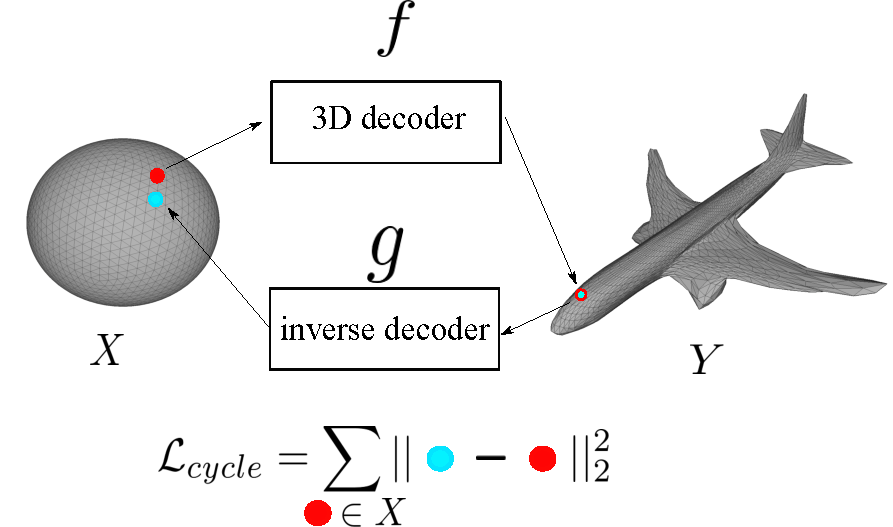
\includegraphics[width=0.48\textwidth]{img/net/cycle}
	\end{center}
	\caption{Illustration of our cycle regularization.}
	\label{fig:cycle}
\end{wrapfigure}
In this section, we firstly establish the relation between self-intersection (means having self-overlapped points on the surface) and non-injectivity.  
Then we introduce the proposed cycle regularization technique and explain in details (as shown in Figure~\ref{fig:net}) about how we respectively apply this general technique onto AtlasNet \cite{atlasnet} and Pixel2Mesh \cite{pixel2mesh}, whose network structures are quite different from each other.

\subsection{Injective Mapping and Self-overlapped Points}
\label{subsec:inj}
Start with the definition of injective mapping at \textbf{Definition}~\ref{def:injective}, we can intuitively induce conclusion that given a surface with $X =\{\mathbf{x}~|~\mathbf{x}$ is a point on the surface$\} $, another surface with $ Y =\{\mathbf{y}~|~\mathbf{y}$ is a point on the surface$\}$ and a function $f:X \rightarrow Y$. If $\exists$ $ \mathbf{a},\mathbf{b} \in X$, $\mathbf{a} \neq \mathbf{b}$ and $f(\mathbf{a}) = f(\mathbf{b})$ (i.e. the overlapped points on target surface exists) then by definition, $f$ is not an injective function. Equivalently (as the converse negative proposition), we can make sure there is no self-overlapped points on the target surface by enforcing injectivity for $f$.
\begin{m_def}
\label{def:injective}
Let $f$ be a function whose domain is a set $X$. The function $f$ is said to be injective provided that
\begin{equation}
\forall \mathbf{a},\mathbf{b} \in X, f(\mathbf{a}) = f(\mathbf{b}) \Rightarrow \mathbf{a} = \mathbf{b}.
\end{equation}
Equivalently, 
\begin{equation}
\forall \mathbf{a},\mathbf{b} \in X, \mathbf{a} \neq \mathbf{b} \Rightarrow f(\mathbf{a}) \neq f(\mathbf{b}).
\end{equation}
\end{m_def}

\subsection{Cycle Regularization}
\label{subsec:cyclereg}
\begin{m_thm}
\label{thm:injective}
A function $f$ with a left inverse is necessarily injective. That is, given $f:X \rightarrow Y$, if there is a function $g:Y \rightarrow X$ such that,
\begin{equation}
\label{equ:injective}
\forall \mathbf{x} \in X,~g(f(\mathbf{x})) = \mathbf{x},
\end{equation}
then $f$ is injective.
\end{m_thm}

Based on \textbf{Theorem}~\ref{thm:injective}, we turn an injective constraint to our cycle regularization term as:
\begin{equation}
\label{equ:cycle_term}
cycle_X(f,g)=\sum_{\mathbf{x}\in X}||g(f(\mathbf{x})) - \mathbf{x}||^2.
\end{equation}
In mesh reconstruction networks, our term can be illustrated as in Figure~\ref{fig:cycle},

By minimizing this term to zero:
\begin{equation}
f^*,g^* = \arg\min_{(f,g)} cycle_X(f,g)
\end{equation}
we can get the $f^*$ that has the left inverse function $g^*$, therefore $f^*$ is injective. 

However, it is almost impossible to actually minimize a regularization term to zero, especially during training neural networks. But when this term is minimized to sufficiently small then we can construct $g^*$ that is the left inverse function of $f^*$ and guarantee that $f^*$ is injective. An example of such case is that when the regularization term is so small that $g(f(\mathbf{x}))$ is closer to $\mathbf{x}$ than any other point in $X$. Such example can be summarized by \textbf{Proposition}~\ref{prop:nearest}.

\begin{m_prop}
	\label{prop:nearest}
	Given sets $X$ and $Y$ that are two subsets of Euclidean space $\mathcal{R}^3$, a function $f:X \rightarrow Y$  and a function $g:Y \rightarrow X$, if
	\begin{equation}
	\exists~g, || g(f(\mathbf{x})) - \mathbf{x} ||^2 \leq \min_{\mathbf{b} \in X}|| g(f(\mathbf{x})) - \mathbf{b} ||^2,
	\end{equation}
	then $f$ is injective.
\end{m_prop}

\textbf{Proposition}~\ref{prop:nearest} can be proved by simply compositing the nearest neighbor with the function $g$. We can construct a nearest neighbor function $l: \mathcal{R}^3 \rightarrow X $ as:
\begin{equation}
\forall \mathbf{a} \in \mathcal{R}^3, l(\mathbf{a}) = \arg\min_{\mathbf{b} \in X} || \mathbf{a} - \mathbf{b} ||^2
\end{equation}
then
\begin{equation}
\begin{aligned}
&|| g(f(\mathbf{x})) - \mathbf{x} ||_2^2 \leq \min_{\mathbf{b} \in X}|| g(f(\mathbf{x})) - \mathbf{b} ||_2^2\\
&\Rightarrow \mathbf{x} = \arg\min_{\mathbf{b} \in X}|| g(f(\mathbf{x})) - \mathbf{b} ||_2^2\\
&\Rightarrow l\Big(g\big(f(\mathbf{x})\big)\Big) = \mathbf{x}\\
\end{aligned}
\end{equation}
then $g^*(\mathbf{y}) = l\big(g(\mathbf{y})\big)$ is the left inverse of $f$, therefore $f$ is injective.

\noindent\textbf{Remaining Gap.}
Even when the condition in Proposition~\ref{prop:nearest} is met after optimization, there is still no guarantee for the injectivity of $f$ over the continuous surface. The reason is that when we turn Eq.~(\ref{equ:injective}) into Eq.~(\ref{equ:cycle_term}), we actually create a theoretical gap. 
The constraint in Eq.~(\ref{equ:injective}) is defined over continuous surface, while the term in  Eq.~(\ref{equ:cycle_term}) is defined on discrete point sets. In order to fill in the gap as much as we can, we randomly sample $X$ from the predefined surface in the training phase instead of minimizing the cycle regularization for any specific set of $X$. Sampling different $X$ from the predefined surface is already employed by AtlasNet. This is a commonly used technique to encode latent variation in generation networks since VAE \cite{VAE}. For Pixel2Mesh, we add such a sampling in the inverse decoding. We did not add it in forward 3D decoding to avoid altering the original forward inference path for Pixel2Mesh. We want to keep our cycle regularization general in the way that it can work along with surface mesh generation networks without altering the original network. Our controlled experiment validates that it is better for our cycle regularization technique to work with such a sampling.

\subsection{Implementation in Networks}

As stated in AtlasNet \cite{atlasnet}, it is possible to use multilayer perceptron with ReLU nonlinearities and enough hidden units to approximate any shape within a small positive error $\epsilon$. In practice, we employ another 3D surface decoder to approximate $g$. Then we explain how we implement this technique for AtlasNet and Pixel2Mesh respectively. Generally speaking, we reuse the network structures from their networks respectively and show that our cycle regularization is generally suitable for this type of networks.

\noindent\textbf{Cycle-AtlasNet} Depending on a shape representing feature $\mathbf{s}$, AtlasNet uses point-wise MLP
$f$ with parameters $\theta_f$ to learn to map points in $X=\{\mathbf{x}| \mathbf{x}$ are points uniformally sampled from surface $P\}$ to points in $Y=\{\mathbf{y}| \mathbf{y}$ are points uniformally sampled from surface $S\}$. In our implementation, $P$ is the surface of a 3D sphere. $S$ is the ground truth surface, which is usually the surface of an object in AtlasNet \cite{atlasnet} and in this paper. Then we use another point-wise MLP $g$ with parameters $\theta_g$ to map points from $Y$ back to $X$. Along with our cycle regularization, the total loss function for Cycle-AtlasNet can be written as:

\begin{equation}
\begin{aligned}
\label{equ:atlascycle}
\mathcal{L}_{(X,Y)}(\theta_f,\theta_g) &= \sum_{\mathbf{x} \in X} \min_{\mathbf{y} \in Y}|| f(\mathbf{x};\mathbf{s},\theta_f) - \mathbf{y} ||^2 \\ &+ \sum_{ \mathbf{y} \in Y}\min_{ \mathbf{x} \in X} || f(\mathbf{x};\mathbf{s},\theta_f) - \mathbf{y} ||^2 \\ &+ \lambda\sum_{\mathbf{x} \in X}||g(f(\mathbf{x};\mathbf{s},\theta_g);\mathbf{s},\theta_f) - \mathbf{x}||^2,
\end{aligned}
 \end{equation}
where the shape representation feature is simply concatenated to each point so that the $f$ and $g$ is depending on a global shape representing feature $\mathbf{s}$. $\lambda$ is the weight for cycle regularization. In AtlasNet, $\mathbf{s}$ is generated from either PointNet \cite{resnet} for auto-encoding or ResNet-18 \cite{resnet} for single view reconstruction. $g$ is a MLP with the same number of units in hidden layers as $f$, as shown in Figure~\ref{fig:net}.

\noindent\textbf{Cycle-Pixel2Mesh}
Comparing to AtlasNet, Pixel2Mesh uses a more complicated network structure which generates shapes in a coarse-to-fine framework. In order to implement cycle regularization along with Pixel2Mesh, we need to cope with such design of network and use the cycle regularization term in each level of point density.
As shown in Figure~\ref{fig:net}, Pixel2Mesh uses three blocks of graph-based convolution residual network ($f_1,f_2,f_3$) to map mesh-based features to the generated surface at three different levels of point density. To be compatible with such a framework, we also use three point-wise MLPs as the inverse decoder and form our regularization term as:
\begin{equation}
\begin{aligned}
\mathcal{L}_{cycle}(\theta_f,\theta_g) 
&= \sum_{\hat{\mathbf{x}} \in \hat{X}_1}||g_{1}(\hat{\mathbf{y_1}};\mathbf{s}_1,\theta_{g_1}) - \hat{\mathbf{x}}||_2^2\\
&+ \sum_{\hat{\mathbf{x}} \in \hat{X}_2}||g_{2}(\hat{\mathbf{y_2}};\mathbf{s}_2,\theta_{g_2}) - \hat{\mathbf{x}}||_2^2\\
&+ \sum_{\hat{\mathbf{x}} \in \hat{X}_3}||g_{3}(\hat{\mathbf{y_3}};\mathbf{s}_3,\theta_{g_3}) - \hat{\mathbf{x}}||_2^2,\\
\end{aligned}
\end{equation}
in which $\hat{\mathbf{x}}$ and $\hat{\mathbf{y}_l}$ are sampled as a convex combination of vertexes in each triangle as:
\begin{equation}
\begin{aligned}
\label{equ:sample}
&\hat{\mathbf{x}} = \sum^{N=3} w_n\mathbf{x}_n, \\
&\hat{\mathbf{y}_l} = \sum^{N=3} w_nf_l(\mathbf{x}_n;\mathbf{s}_l,\theta_{f_l}),\\
&\sum^{N=3} w_n = 1.
\end{aligned}
\end{equation}
The combination coefficients $w_n$ are randomly generated but kept the same for corresponding $\hat{\mathbf{x}}$ and $\hat{\mathbf{y}_l}$ in each level $l$. $\theta_f$ is the whole parameters for $f_1,f_2,f_3$. $\theta_g$ is the whole parameters for $g_1,g_2,g_3$. $\mathbf{s}_1,\mathbf{s}_2,\mathbf{s}_3$ are features extracted from different layers of VGG-16 based on input point positions $X_1,X_2,X_3$ in the network. $\hat{X}_1,\hat{X}_2,\hat{X}_3$ are the sets of sampled points at each level.
As mentioned in Sec~\ref{subsec:cyclereg}, random sampling from predefined surface is crucial for our technique. Since Pixel2Mesh does not include such sampling in their method, we add it in our inverse decoding. In other words, in our inverse decoding we do not directly map the vertices from the target surface back to the predefined surface. Instead, we map the sampled points $\hat{\mathbf{y}_l}$ from each face back to the corresponding samples $\hat{\mathbf{x}}$. The correspondence between $\hat{\mathbf{x}}$ and $\hat{\mathbf{y}_l}$ are ensured to be locally injective by using the same set of convex combination coefficients $w_n$ for the sampling. We multiply our regularization term with weight $\lambda$ and add it to original loss function of Pixel2Mesh (see \cite{pixel2mesh} for original loss function). For more details of our implementation, please go to our supplemental material for the code.
